\documentclass[11pt]{scrartcl}
\usepackage{tikz}
\usetikzlibrary{%
  arrows,
  calc
}
\tikzset{>=latex}
\begin{document}
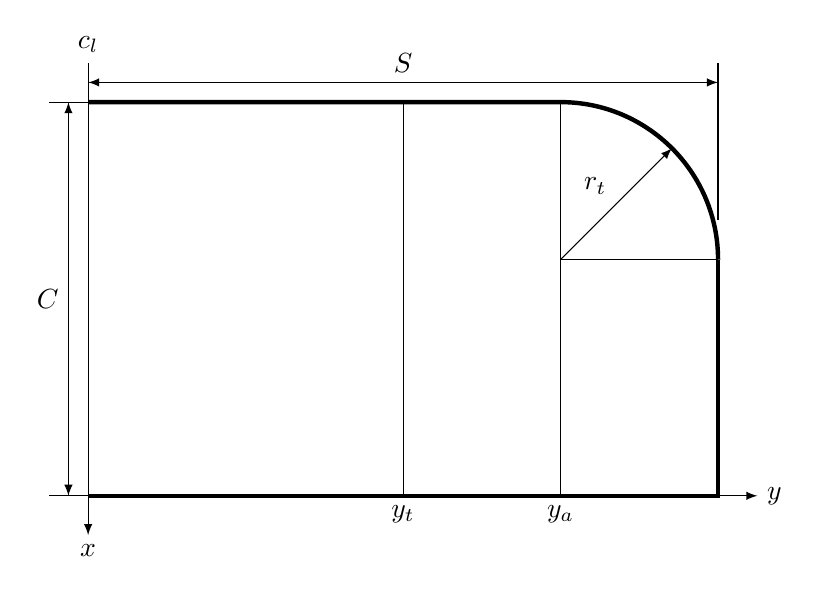
\begin{tikzpicture}


  \draw[ultra thick]  (0,0) -- (8,0) -- (8,3);
  \draw[ultra thick]  (8,3) arc[
  start angle=0,
  end angle=90,
  x radius=2,
  y radius=2] -- (0,5);

\draw[thin] (0,5) -- (0,5.5) node[above] {$ c_l $};
  \draw[thin] (0,0) -- (0,5);
  \draw[thin,->] (0,0) -- (0,-0.5) node [below] {$x$};

  \draw[thin] (4,5) -- (4,0) node[below] {$y_t$};

  \draw[thin] (6,5) -- (6,0) node[below] {$y_a$};
  \draw[thin] (6,3) -- (8,3);
  \draw[thin,->] (8,0) -- (8.5,0) node[right] {$y$};

  \draw[thin] (0,0) -- (-0.5,0);
  \draw[thin] (0,5) -- (-0.5,5);
  \draw[thin,<->] (-0.25,0) -- node[left] {$C$}(-0.25,5);

  \draw[thin,->] (6,3) --node[above left] {$r_t$}  +(45:2);

  \draw[thin] (8,3.5) -- (8,5.5);
  \draw[thin, <->] (0,5.25) -- node[above] {$S$}(8,5.25);

\end{tikzpicture}
\end{document}
